\section{Problemas}

\subsection{Estimación de Pose en Humanos}

La tarea de \textit{Estimación de Pose en Humanos} ha sido uno de los tópicos de gran importancia en
el campo de Visión por Computadora. Debido a la búsqueda de automatización y entendimiento de
diversas actividades humanas, sus utilidades causan impacto directo en las implementaciones
tecnológicas del mundo real, tales como, la predicción de intención (vigilancia), sistemas de
autónomos y de asistencia en la conducción automóviles, animación, simulaciones,
interacción Humano-Computadora (HCI), realidad virtual
aumentada (VR y AR), videojuegos, salud o asistencia médica o hasta análisis de movimiento en
deportes. La tarea de \textit{Estimación de Pose} no solo se limita a el cuerpo
humano, también, puede ser empleado en objetos como carros o animales, vease la imagen \ref{fig:PE-track}.

Con el crecimiento acelerado de \textit{Aprendizaje Profundo} en los últimos años gracias a las
capacidades actuales de potencia de cómputo los métodos basados bajo este enfoque han sobrepasado
a las métodos tradicionales, sin embargo aún existen distintos problemas y retos que siguen presentes
como la oclusión y la ambiguedad de los datos o la dificultad de su obtención para realizar
entrenamientos.

\begin{figure}[ht!]
    \centering
    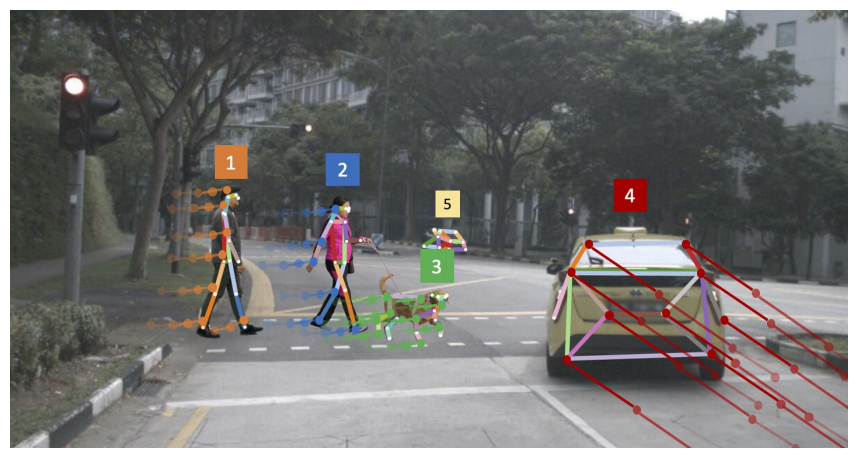
\includegraphics[width=0.4 \textwidth]{Chapters/1. Pose Estimation/figures/openpifpaf.png}
    \caption{OpenPifPaf: Escena del mundo real desde la perspectiva de un carro autónomo. Todos los actores
             son detectados y seguidos, esto incluye a las personas, el carro y el perro. \cite{DBLP:journals/corr/abs-2103-02440}}
    \label{fig:PE-track}
\end{figure}


El problema de \textit{Estimación de Pose Humanos} consiste en predecir las partes del cuerpo o las
posiciones de las articulaciones de una persona a través de una imagen, video. Este problema ha sido
cuidadosamente estudiado a lo largo de los años y diversas recopilaciones de investigaciones han sido escritas.
En la tabla \ref{Tab:hpe-survey} se resumen algunas de las más recientes y que describen dos formas
generales de abordar el problema. La primera de ellas la \quotes{Tradicionalista}, cuyos métodos
usan enfoques clásicos de visión por computadora o la segunda basada en técnicas de aprendizaje
profundo que involucran comúnmente modelos convolucionales. El trabajo realizado en esta tesis está
basado en el segundo método, usando técnicas de aprendizaje profundo y modelos actuales capaces
de capturar información temporal, específicamente enfocado en modelos \textit{Transformers} \cite{Vaswani}.

\begin{table}[ht!]
    \begin{center}
    \resizebox{\textwidth}{!}{%
    \begin{tabular}{|l|l|l|l|}
        % \hline
        % \multicolumn{4}{|c|}{Recopilaciones} \\
        \hline
        \multirow{2}*{\textbf{Título}} & \multirow{2}*{\textbf{Año}} & \textbf{Métodos} & \multirow{2}*{\textbf{Descripción}}\\
         & & \textbf{cubiertos} & \\
        \hline
        \multirow{2}*{A survey of computer vision-based motion capture \cite{MOESLUND2001231}} & \multirow{2}*{2001} & \multirow{2}*{Tradicionales} &  Investigacion general sobre métodos de captura de movimientos basados en visión en\\
        & & & humanos. Incluye estimación de pose, seguimiento y reconocimiento de acciones. \\\hline

        A survey of advances in vision-based human motion capture and analysis \cite{MOESLUND200690} & 2006 & Tradicionales & Incluye una revisión de los métodos de captura de movimiento del año 2001 al 2006.\\ \hline

        \multirow{2}*{Vision-based human motion analysis: An overview. \cite{POPPE20074}} & \multirow{2}*{2007} & \multirow{2}*{Tradicionales} & Investigacion general sobre métodos de captura de movimientos usando datos \\
        & & & sin marcadores de dispositivos de captura. \\\hline

        \multirow{2}*{Advances in view-invariant human motion analysis: A review \cite{5191035}} & \multirow{2}*{2010} & \multirow{2}*{Tradicionales} & Estudio de métodos de estimación de pose en 3D, comportamiento y \\
        & & & reconocimiento/representación de acciones. \\ \hline

        Human pose estimation and activity recognition from multi-view videos: & \multirow{2}*{2012} & \multirow{2}*{Tradicionales} & Métodos de estimación de pose 3D y reconocimiento de acción usando datos \\
        Comparative explorations of recent developments \cite{6193117} &  &  & multi-vista\\ \hline

        A survey of human pose estimation: the body parts parsing based methods \cite{LIU201510} & 2015 & Tradicionales & Estudios de estimación de pose enfocados principalmente a las técnicas de localización \\
        & & & de las distintas partes del cuerpo. \\ \hline

        \multirow{2}*{Human pose estimation from monocular images: A comprehensive survey \cite{Gong2016}} & \multirow{2}*{2016} & \multirow{2}*{Ambos} & Enfocado en la estimación de pose usando datos monoculares incluyendo las\\
        & & & metodologías usadas en procesos tradicionales y basados en aprendizaje profundo. \\ \hline

        \multirow{2}*{3D human pose estimation: A review of the literature and analysis of covariates \cite{SARAFIANOS20161}} & \multirow{2}*{2016} & \multirow{2}*{Deep-Learning} & Revisión general del estado del arte de estimación de pose 3D usando imágenes\\
        & & & y videos RGB. \\ \hline

        \multirow{2}*{Monocular human pose estimation: a survey of deep learning-based methods \cite{CHEN2020102897}} & \multirow{2}*{2020} & \multirow{2}*{Deep-Learning} & Revisión y clasificación general de los métodos de estimación de pose basados en \\
        & & & aprendizaje profundo desde el 2014 usando solo datos monoculares.\\ \hline

        The progress of human pose estimation: a survey and taxonomy \cite{9144178} & \multirow{2}*{2020} & \multirow{2}*{Deep-Learning} & Revisión de los métodos basados en aprendizaje profundo para estimación de \\
        of models applied in 2D human pose estimation &  & & pose 2D\\ \hline

        Deep Learning-Based Human Pose Estimation: A Survey \cite{DBLP:journals/corr/abs-2012-13392} & 2020 & Deep-Learning & Estudio general del estado del arte de estimación de pose 2D y 3D.\\ \hline
    \end{tabular}}
    \end{center}
    \caption{Listado de diversas investigaciones de \textit{Estimación de Pose en Humanos} que abarcan
             tanto enfoques tradicionales como basados en aprendizaje profundo.
             Tabla basada en el trabajo de \citeauthor*{DBLP:journals/corr/abs-2012-13392}.}
    \label{Tab:hpe-survey}
\end{table}

\subsubsection{Directrices de estimación de Pose 2D y 3D}


\begin{tikzpicture}[
    mindmap,
    concept color = red!30,
    every node/.style = {concept},
    grow cyclic,
    level 1/.append style = {
        level distance = 4.5cm,
        sibling angle = 120
    },
    level 2/.append style = {
        level distance = 3cm,
        sibling angle = 45}
]

\node {Our root concept}
    child {node [concept color = blue!30] {First idea}
        child {node {Fact 1}}
        child {node {Fact 2}}
    }
    child [concept color = green!30] {node {Second idea}
        child {node {Sub-idea}}
    }
    child {node [concept color = magenta!30] {Third idea}
            child [concept color = magenta!50!black] {node {Note 1}}
            child [concept color = magenta!60!black] {node {Note 2}}
            child [concept color = magenta!70!black] {node {Note 3}}
    };

\end{tikzpicture}

Depending on the output dimension requirement, the Pose Estimation problem can be classified into
2D Pose Estimation and 3D Pose Estimation. 2D Pose Estimation is predicting the location of body
joints in the image (in terms of pixel values). On the other hand, 3D Pose Estimation is predicting
a three-dimensional spatial arrangement of all the body joints as its final output.

2D Pose Estimation vs 3D Pose Estimation
Most 3D Pose Estimation models first predict 2D Pose, and then try to lift it to 3D Pose. However,
some end-to-end 3D Pose Estimation techniques also exist which directly predict 3D Pose.


The major challenges for tracking poses from the car perspective are
(i) occlusions due to the viewing angle and (ii) prediction
speed to be able to react to real-time changes in the environ

Biased databases
La mayoría de la bases de datos son obtenidas a través de algunos pocos sujetos de prueba.
La estructura fisiológica de individuos no es perfecta y pueden variar debido a diversos factores
como el sexo, la raza, edad, lugar de nacimiento y desarrollo, enfermedades, factores genéticos, entre
otros, además de que los movimientos recreados entre sujetos no siempre son recreados de la misma manera
aunque las circunstancias o ambiente esté controlado.

Irregularidades en los datos reales.
Si los datos son obtenidos bajo un ambiente controlado es posible obtener imágenes fieles para el
entrenamiento. Por otro lodo, los modelos al ser desplegados y puestos en marcha en ambientes reales
se enfrentan a imprevistos de los que no se puede tener control; oclusiones de diversas partes del
cuerpo ya sea por el mismo sujeto o algún objeto extraño en la captura, movimientos extraños o rápidos
como correr o dar una patada donde el modelo no puede los puede identificar o el equipo de captura
no pueda obtener que se ven como fotogramas borrosos.

Monocular human pose estimation has some unique characteristics
and challenges:

Flexible body configuration indicates complex interdependent
joints and high degree-of-freedom limbs, which may cause self occlusions or rare/complex poses.
- Diverse body appearance includes different clothing and self similar parts.
- Complex environment may cause foreground occlusion, occlusion
or similar parts from nearby persons, various viewing angles, and
truncation in the camera vie


Problem Clasification by axes


- Number of People Being Tracked

Depending on the number of people being tracked, pose estimation can be classified into
Single-person and Multi-person pose estimation

Single-person pose estimation (SPPE) is the easier of the two, with the guarantee of only one person
present in the frame. On the other hand, Multi-person pose estimation (MPPE) needs to handle the
additional problem of inter-person occlusion. Initial approaches in pose estimation were mostly
focused on SPPE, however with the availability of huge multi-person datasets, the MPPE problem has
lately been getting increased attention.

- Input Modality

Red-Green-Blue (RGB) image : The images that we see around us on a daily basis, and the most common
type of input for Pose Estimation. Models working on RGB-only input have a huge advantage over
others in terms of the mobility of the input source. This is due to the ease of availability of
common cameras (which capture RGB images), making them the models that can be used across a huge
number of devices.

Depth (Time of Flight) image : In a Depth image, the value of a pixels relates to the distance from
the camera as measured by time-of-flight. The introduction and popularity of low-cost devices
like Microsoft Kinect has made it easier to obtain Depth data. Depth image can complement RGB image
to create more complex and accurate Computer Vision models, whereas Depth-only models are vastly
used where privacy is a concern.

Infra-red (IR) image : In an IR image, the value of a pixel is determined by the amount of infrared
light reflected back to the camera. Experimentation in Computer Vision based on IR images are minimal,
as compared to RGB and Depth images. Microsoft Kinect also provides IR image while recording.
However, currently there are no datasets that contain IR images.

Static Image vs Video

A video is nothing but a collection of images, where every two consecutive frames share a huge
portion of the information present in them (which is the basis of most of the video compression
techniques). These temporal (time based) dependence in videos can be exploited while performing
Pose estimation.
For a video, a series of poses need to be produced for the input video sequence. It is expected
that the estimated poses should ideally be consistent across successive frames of video, and the
algorithm needs to be computationally efficient to handle large number of frames. The problem of
occlusion might be easier to solve for a video due to the availability of past or future frames
where the body part is not occluded.

If temporal features are not a part of the pipeline, it is possible to apply static pose estimation
for each frame in a video. However, the results are generally not as good as desired due to jitters
and inconsistency problems.

Body Model
Every pose estimation algorithm agrees upon a body model beforehand. It allows the algorithm to formalize the problem of human pose estimation into that of estimating the body model parameters. Most algorithms use a simple N-joint rigid kinematic skeleton model (N is typically between 13 to 30) as the final output. Formally, kinematic models can be represented as a graph, where each vertex V represents a joint. The edges E can encode constraints or prior beliefs about the structure of the body model.
Such a model suffices for most applications. However, for many other applications such as character animation, a more elaborate model may be needed. Some techniques have considered a highly detailed mesh models, representing the whole body with a point cloud.
Another rather primitive body model that was used in earlier Pose Estimation pipelines is a shape-based body model. In shape-based models, human body parts are approximated using geometric shapes like rectangles, cylinders, conics etc.

kinematic Model
Planar Model
Volumetric Model
-> https://viso.ai/deep-learning/pose-estimation-ultimate-overview/

Number of cameras
A major portion of research involves solving the pose estimation problem using input from a single camera. However, there are certain algorithms which try to use data from multiple viewpoints/cameras, combining them to generate more accurate poses and handle occlusions better. The research on multi-camera pose estimation is currently somewhat limited, primarily due to lack of good datasets.

Mapa de tipos de estimación de pose 3D
-> https://sci-hub.se/10.1016/j.cviu.2019.102897 pp 4

Why is it hard?
Strong articulations, small and barely visible joints, occlusions, clothing, and lighting changes make this a difficult problem.
Main challenges -> https://viso.ai/deep-learning/pose-estimation-ultimate-overview/

Pipelines

-> https://towardsdatascience.com/human-pose-estimation-simplified-6cfd88542ab3

Approaches

- Classical approaches
- Deep Learning based approaches
-> https://nanonets.com/blog/human-pose-estimation-2d-guide/
- Bottom-up
- Top-Down
-> https://viso.ai/deep-learning/pose-estimation-ultimate-overview/


Most popular pose estimation methods
-> https://viso.ai/deep-learning/pose-estimation-ultimate-overview/


datasets
-> https://sci-hub.se/10.1016/j.cviu.2016.09.002

Modern pose estimation algorithms are almost exclusively based on convolutional neural networks with hourglass architecture or its variants (see the image below). Such a network consists of two major parts: a convolutional encoder that compresses the input image into the so-called latent representation and decoder that constructs N heatmaps from the latent representation where N is the number of searched keypoints.




\subsection{Lung Pathologies detection}
